%! TEX root = main.tex

%/========== Introduction ==========/%

\chapter{Introduction}

The Estonian sport of \textit{Kiiking} (Figure \ref{fig:kiiking}) is the adult
equivalent of a child playing on a standing swing, though here
an athlete attempts to make a giant solid steel swing gain momentum.
Naturally, the kiiker begins by pushing off the ground and proceeds to alternate
between standing and squatting. 
This allows them to swing higher and faster over time, until they have reached
their express goal of spinning at high speed around the bar.

\begin{figure}[ht]
    \centering
    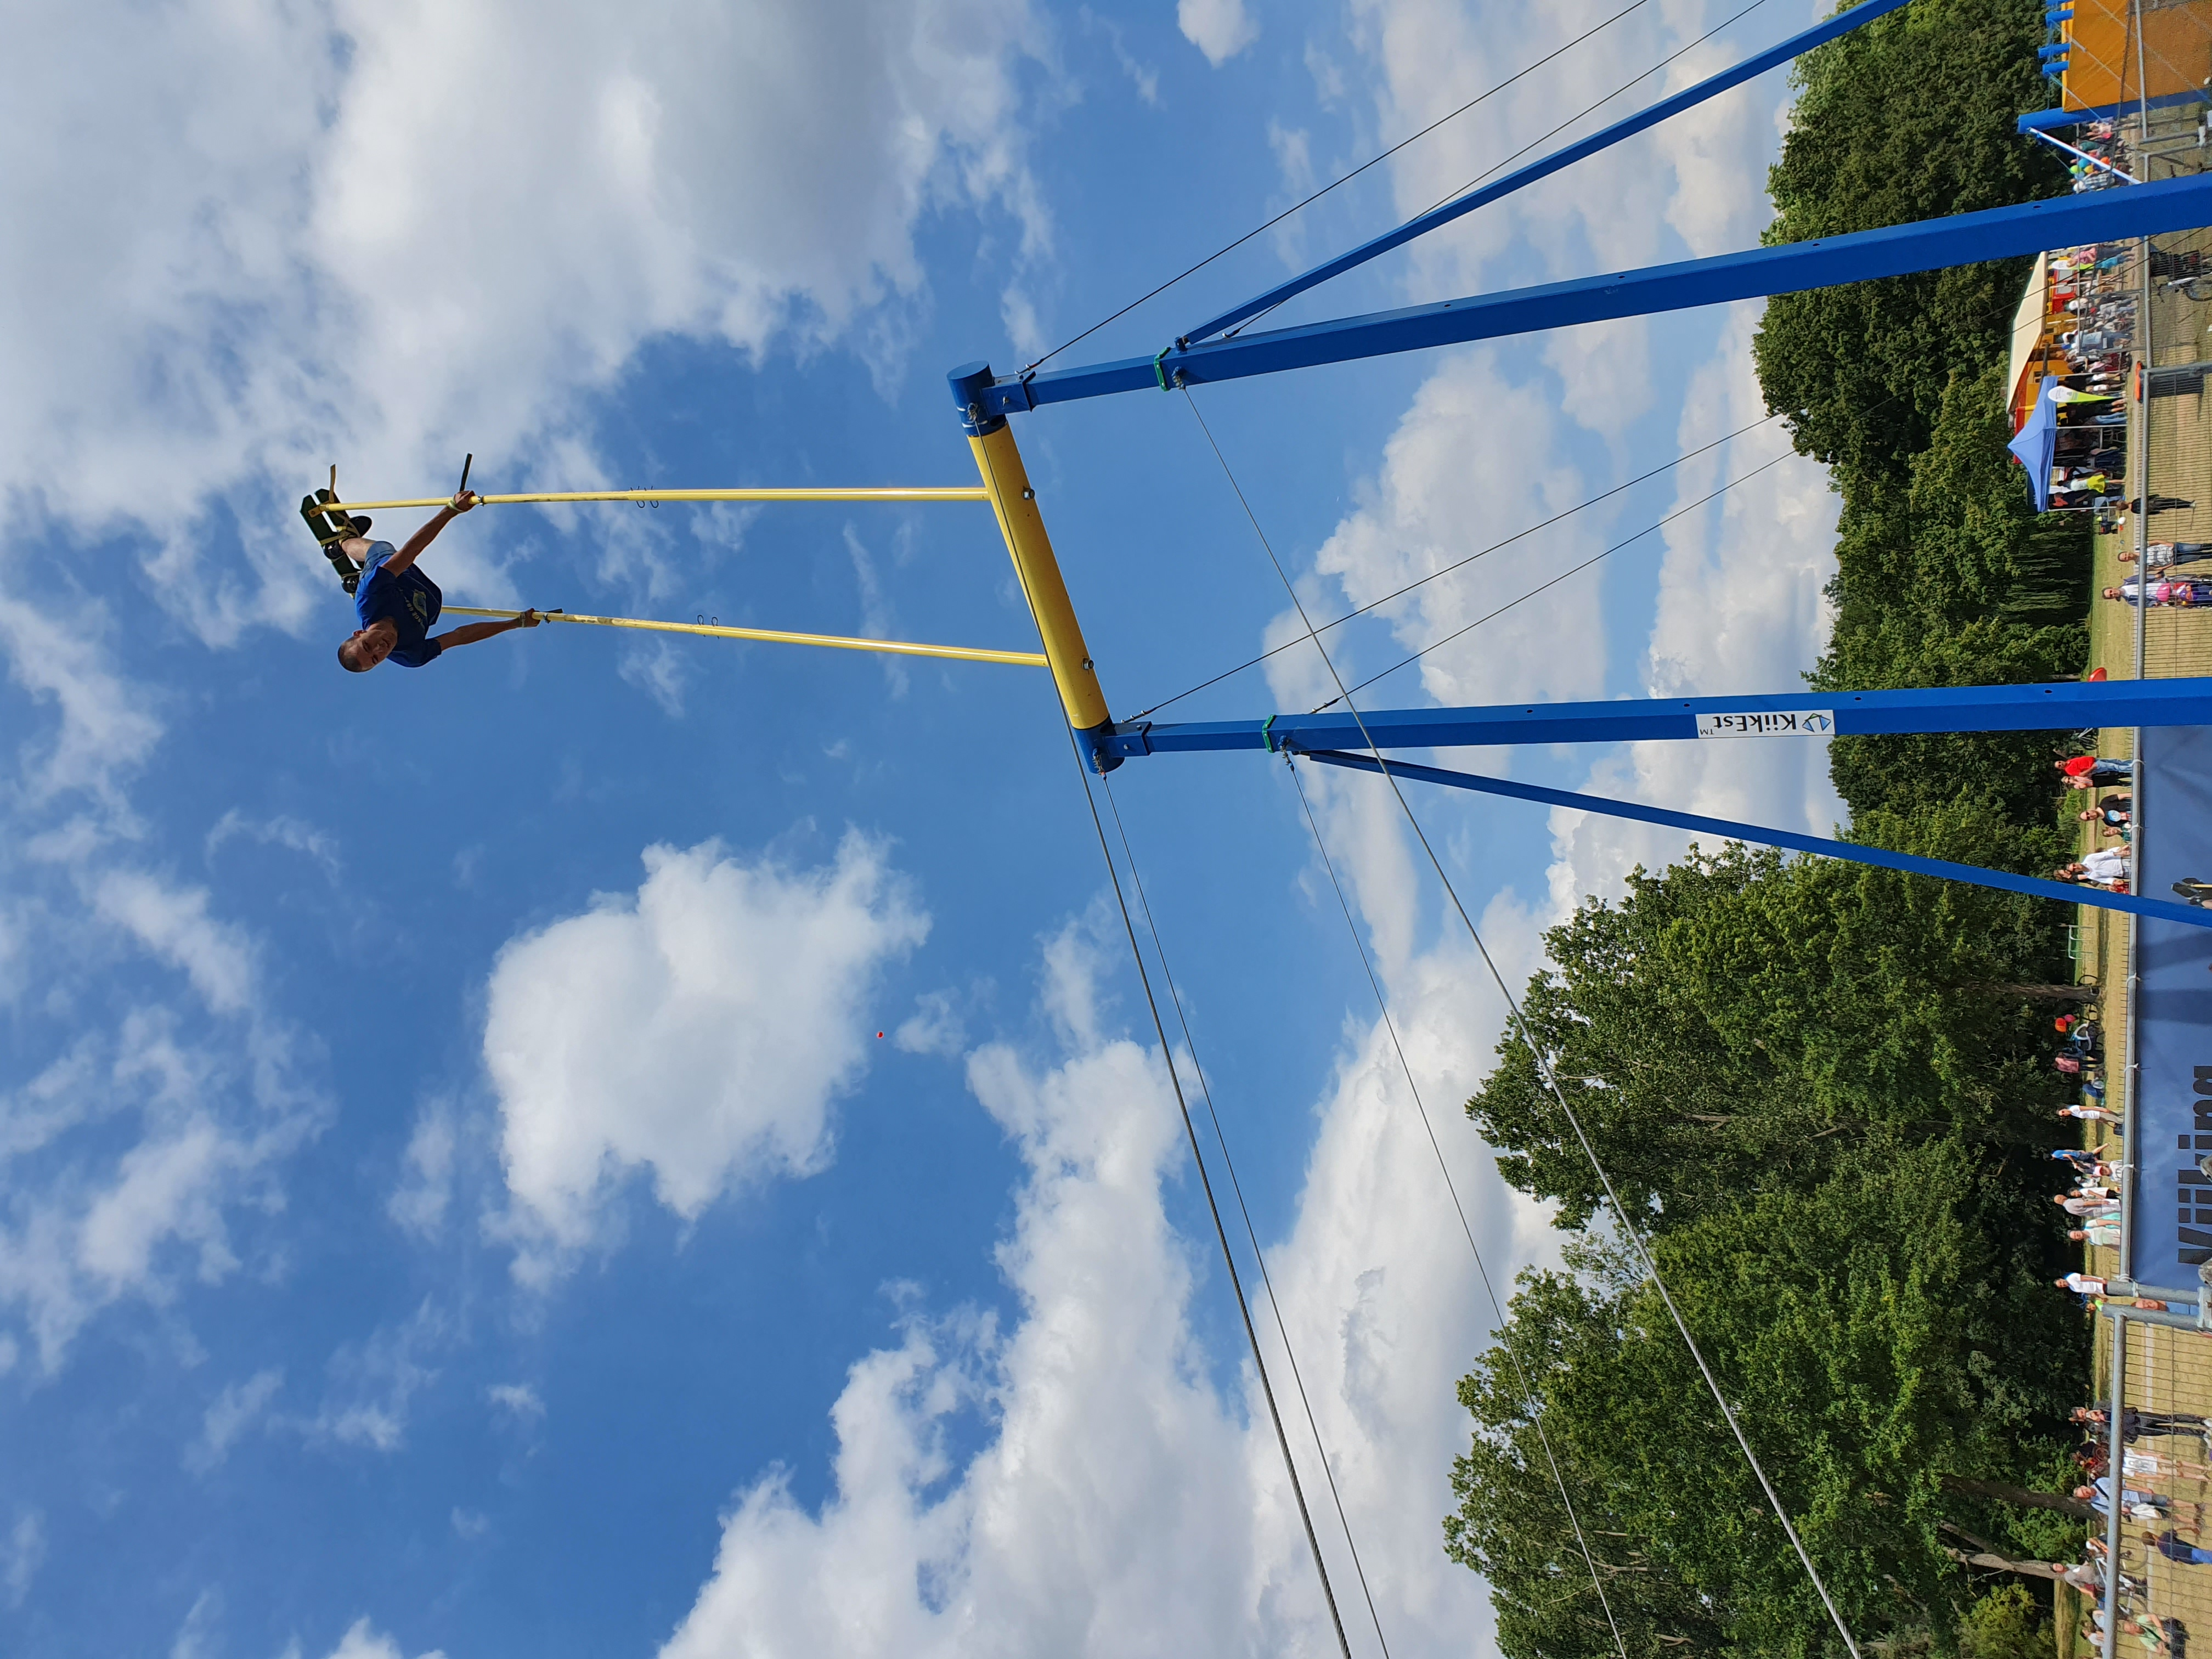
\includegraphics[width=0.6\textwidth,angle=270]{images/kiiking.jpg}
    \caption{Kiiking, which translates to ``swing", involves a person standing
        and squatting on a giant swing until they are rotating around the bar.
    Image taken from \cite{kiiking-img}.}
    \label{fig:kiiking}
\end{figure}

Now imagine that the kiiker is a robot, and their creator is teaching them to
swing like a human.
If the roboticist had studied classical control theory, they would plot 
a kiiker's squat depth as a trajectory over time and tell the robot to
synchronize with this trajectory.
In an ideal world, this technique would work perfectly; unfortunately, it is
also entirely unnatural. 
After all, humans on swings do not have an internal stopwatch telling them when
to squat.
Rather, they adjust how much they bend their knees based on the current angle of
the swing along with their direction of motion.
This position-velocity adjustment allows humans to correct for external
disturbances (like strong winds or enthusiastic swing pushers). 
Figure \ref{fig:swing-pos-vel} shows this adjustment process:
a person will squat when they reach the peak of their swing, and
stand when they reach the fastest point at the bottom
\cite{pumping_swing_standing_squatting}.
Even if the robot could perfectly track a time-based trajectory, an external
disturbance may affect where squatting and standing occurs to the point that
the swing actually slows down.

\begin{figure}
    \centering
    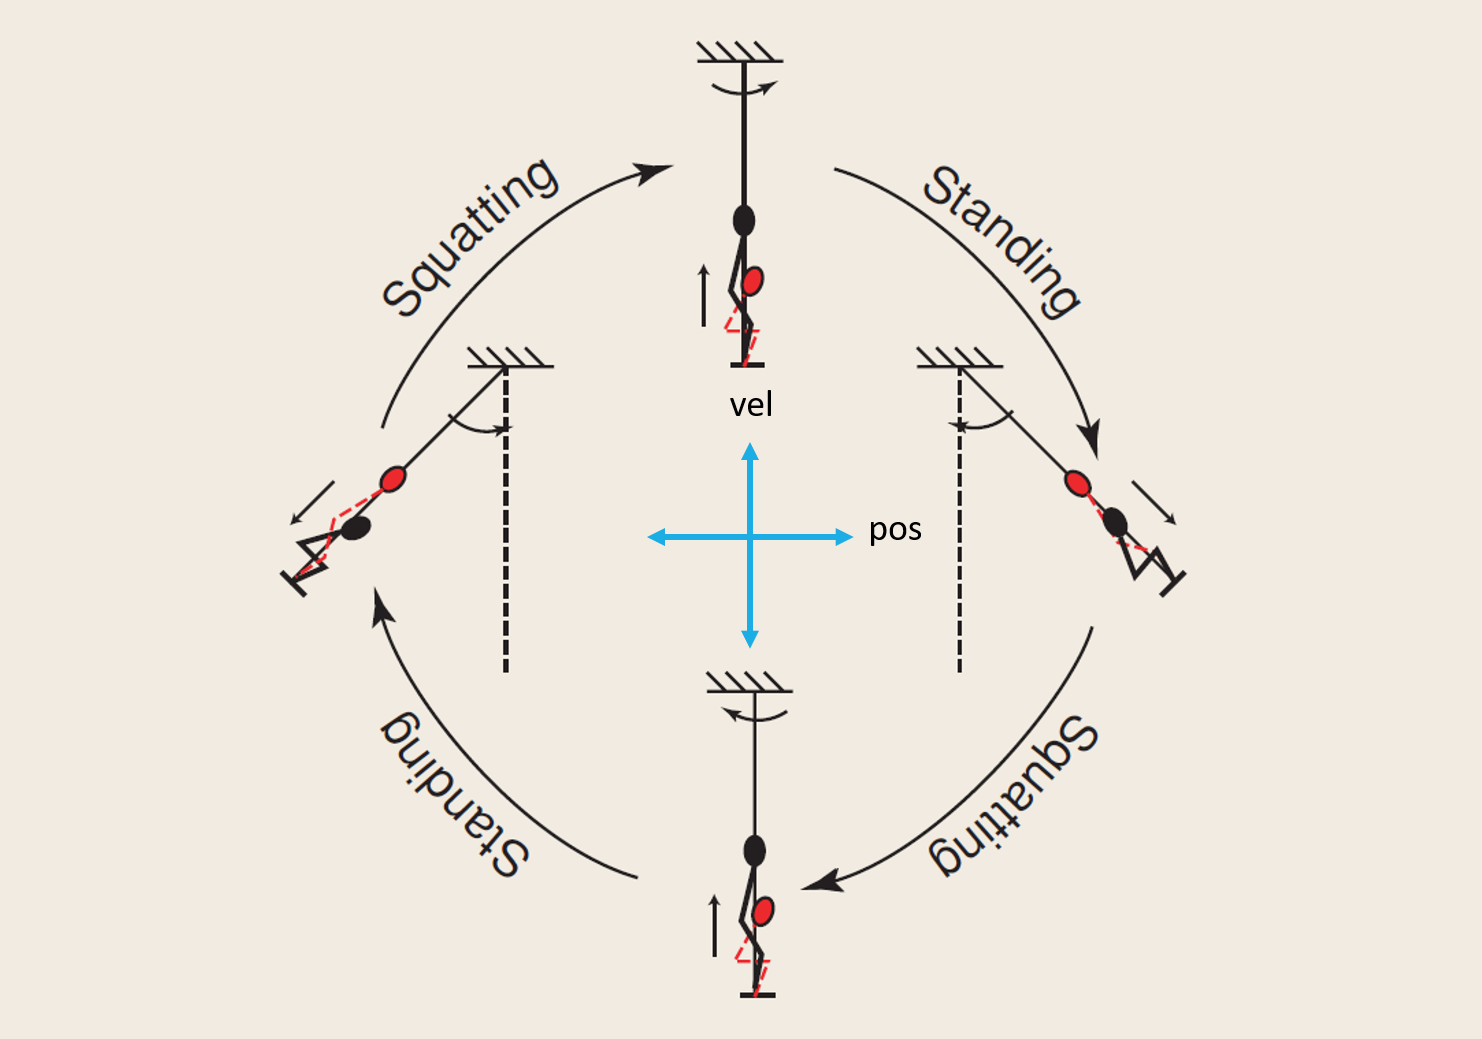
\includegraphics[width=0.75\textwidth]{images/swing_pos_vel.png}
    \caption{A person on a standing swing will stand at the bottom of the swing
        arc, and squat at the top. Figure modified from
        \cite{pumping_swing_standing_squatting}.}
    \label{fig:swing-pos-vel}
\end{figure}

To fix this issue, a clever roboticist might use \textit{virtual holonomic
constraints}, which are controllers that track a function of position rather
than time \cite{vhcs_for_el_systems}.
Sadly, this still fails since one needs velocity to determine when they
have reached the peak of their swing.
In other words, the robot needs to move according to a function of both position
and velocity if it has any hope of behaving like a real person.
These position-velocity controllers are known as 
\textit{virtual nonholonomic constraints}, and they are the focus of this
thesis.

Our goal throughout this thesis is to prove that virtual
nonholonomic constraints can increase a robot's momentum through a
process known as \textit{energy injection}.
We will use two benchmark robotic systems to build intuition and test
our theory.
The first system is the variable-length pendulum, which models a person
on a swing.
The second is the acrobot, an actuated double pendulum which models a gymnast
hanging on a horizontal bar.
For each of these examples, we will create virtual nonholonomic
constraints which model human motion and will rigorously prove that these
constraints inject energy. 

\section{Literature Review}
Let us review some of the existing research on energy injection and virtual
nonholonomic constraints.

Energy injection for mechanical systems is often performed by passivity-based
control and energy shaping --- one views the robot and its inputs as energy
transformations which are moulded to enforce desired behaviour.
Much of the theoretical work in this field has been performed by Ortega, van der
Schaft, and others (see for example \cite{ida_pbc_underactuation_one,
ida_pbc_acrobot_example,energy_shaping_revisited}).
Energy shaping has been applied to both the variable-length
pendulum \cite{vlp_energy_shaping} and the acrobot
\cite{swingup_acrobot_energy,swingup_giant_acrobot}.
This technique is useful and widely applicable, but it does not
produce the structured human-like motion we wish to generate using virtual
nonholonomic constraints.

The modern concept of virtual nonholonomic constraints was described by
\citet{nhvc_dynamic_walking} in 2015, though there are references to more
primitive versions going back as early as the the year 2000
\cite{vnhc_human_robot_cooperation}.
Virtual nonholonomic constraints have been of most notable use in
bipedal locomotion 
\cite{nhvc_gait_optimization,output_nhvc_bipedal_control},
where they have shown marked improvements in the robustness of walking gaits
when compared to previous control techniques.
They have also been used for error-reduction in time-delayed teleoperation
\cite{vnhc_time_delay_teleop} and in the field of human-robot interaction
\cite{psd_based_vnhc_redundant_manipulator,haptic_vnhc}.
\citet{hybrid_zero_dynamics_bipedal_nhvcs} have derived the 
zero dynamics for hybrid mechanical systems under virtual nonholonomic
constraints.
In particular, they study a class of constraints formed by taking an affine
sum of holonomic functions with nonholonomic B\'{e}zier polynomials.
They widen this class of constraints in \cite{nhvc_incline_walking} to improve
bipedal locomotion on variable-slope terrain, and generate constraints through
a specialized optimization routine.

The most recent literature surrounding virtual nonholonomic constraints
has focused on enforcing stable periodic orbits for hybrid mechanical systems
with impacts.
To the best of our knowledge, no one has studied how virtual nonholonomic
constraints can be used for energy injection, where periodic motion is not
desirable.
This thesis attempts to fill this gap in the research.
For more detail on the differences between this thesis and the existing research
on virtual nonholonomic constraints, see Chapter \ref{ch:vnhc-compare}.

Many of the contributions in this thesis are extensions of concepts from the
field of virtual holonomic constraints. 
Of note is the framework devised by Mohammadi, Maggiore, and
Consolini, among others
\cite{vhcs_for_el_systems,dynamic_vhcs_stabilize_closed_orbits,lagrangian_structure_reduced_dynamics_vhcs,xingbo_thesis}.

\section{Statement of Contributions}
Here are the contributions of this thesis.
\begin{itemize}[label={}]
   \item \textbf{Chapter \ref{ch:vnhcs}} The development of 
      virtual nonholonomic constraints.
      This includes the definition of simply actuated mechanical systems, virtual
      nonholonomic constraints, regular constraints, and energy injection.
      Theorem \ref{thm:vnhc-regularity} yields a computational characterization
      of regularity, while Theorem \ref{thm:zero-dynamics} explicitly finds the
      constrained dynamics for a certain class of systems.
   \item \textbf{Chapter \ref{ch:vlp}} An application of virtual nonholonomic
      constraints to the variable-length pendulum, based on a pumping technique
      used by children on standing swings.
      The chapter culminates in Theorem \ref{thm:vlp-energy-stabilization},
      which guarantees that a certain class of VNHCs will inject energy into
      this system.
   \item \textbf{Chapter \ref{ch:acrobot}} An application of virtual
      nonholonomic constraints to the acrobot, based on the motion performed by
      human gymnasts.
      The chapter ends with Theorem \ref{thm:acrobot-energy-stabilization},
      which proves that the constraint we design does in fact inject energy into
      the acrobot.
\end{itemize}

\section{Organization of the Thesis}
The thesis is laid out as follows: 
in Chapter \ref{ch:vnhcs} we cover the requisite background on analytical 
mechanics, after which we develop the main theory of virtual nonholonomic
constraints;
in Chapter \ref{ch:vlp} we reformulate a time-optimal energy-injection strategy
for the variable-length pendulum as a virtual nonholonomic constraint, and
prove that the pendulum will gain enough energy to rotate around the bar with
arbitrary speed;
and in Chapter \ref{ch:acrobot} we find a virtual nonholonomic constraint 
which enables the acrobot to kick its legs like a gymnast until it
performs backflips on a horizontal bar.
Finally, we show experimental results on a physical acrobot which confirm
that the theory works in the real world.

%/========== /Introduction ==========/%
% vim: set tw=80 ts=4 sw=4 sts=0 et ffs=unix :
